% \documentclass[rmp,aps,floatfix,authordate1-4,preprint]{revtex4}
% \documentclass[prb,aps,floatfix,authordate1-4,preprint]{revtex4}

\documentclass[pre,aps,floatfix,authordate1-4,twocolumn]{revtex4-1}
%\documentclass[pre,aps,floatfix,authordate1-4]{revtex4-1}

%\documentclass[aps,prl,preprint,superscriptaddress]{revtex4}



%\documentclass[aps,prl,preprint,groupedaddress]{revtex4}

\usepackage{rotating} 
\usepackage{times}
\usepackage{graphicx}
\usepackage{setspace}
\usepackage{amsmath}
\usepackage{caption}
\usepackage{subcaption}
%\usepackage{array}
\usepackage{arydshln}
%\usepackage[sort&compress]{natbib}
%\bibpunct{(}{)}{,}{n}{}{}
%\renewcommand{\bibnumfmt}[1]{#1.}
\usepackage[obeyFinal]{easy-todo}

\begin{document}
%\singlespacing

\title{Binding of cations to phospholipid bilayers}

\author{Andrea Catte}
\thanks{The authors are listed in alphaphetical order.}
\thanks{The author list is not completed.}
\thanks{University of East Anglia, Norwich, United Kingdom}
\author{Matti Javanainen}
\thanks{Tampere University of Technology, Tampere, Finland}
\author{Markus S. Miettinen}
\thanks{Fachbereich Physik, Freie Universit\"at Berlin, Berlin, Germany}
\author{Luca Monticelli}
\thanks{Institut de Biologie et Chimie des Prot{\'e}ines (IBCP), CNRS UMR 5086, Lyon, France}
%\setcounter{page}{1}
\author{Vasily S. Oganesyan}
\thanks{University of East Anglia, Norwich, United Kingdom}
\author{O. H. Samuli Ollila} 
\thanks{{\bf Author to whom correspondence may be addressed. E-mail: samuli.ollila@aalto.fi.}}
\thanks{Helsinki Biophysics and Biomembrane Group, Department of Biomedical Engineering and Computational Science, Aalto University, Espoo, Finland}
%\footnote{Author to whom 
%correspondence may be addressed. E-mail: samuli.ollila@aalto.fi.\\
%}
%\affiliation{
%  Helsinki Biophysics and Biomembrane Group,
%Department of Biomedical Engineering and Computational Science, Aalto University, Espoo, Finland
%}



\begin{abstract}
%We compare the order parameters predicted for the hydrocarbon segments in lipid bilayer headgroup region
%by the Berger molecular dynamics simulation model to those measured by Nuclear Magnetic Resonance (NMR) experiments.
%We first show results for a fully hydrated POPC bilayer, and then focus on changes of the order parameters as
%a function of hydration level, NaCl and CaCl$_2$ concentrations, and cholesterol content. The experimental headgroup order 
%parameters are never reproduced.
%This indicates that under all of these conditions the used model is unable to correctly reproduce the headgroup structure. 
%Consequently, many of the conclusions drawn over the years from this model might be erroneous.
%This manuscript has not been submitted to any journal, instead its contents are discussed at 
%nmrlipids.blogspot.fi.
Despite of vast amount of experimental and theoretical studies the binding affinity of cations, especially biologically relevant Na$^+$ and Ca$^{2+}$ ions,
into a phosholipid bilayer is not agreed in the literature. Here we directly compare the measured choline headgroup order parameters
to the simulations with different models in the presence of different cations. We conclude that the least complicated explanation
for the experimental and theoretical observations is that the Na$^+$ ions do not penetrate into a phosphatidylcholine lipid
bilayer in mM concentrations, in contrast to Ca$^{2+}$. Further, the binding affinity of Na$^+$ is overestimated in almost all molecular dynamics simulation models.
However, the electrometer concept connecting the choline order parameter changes to the penetrating charges is valid also in simulations.
This work has been, and continues to be, progressed and discussed through the blog: nmrlipids.blogspot.fi.
Everyone is invited to join the discussion and make contributions through the blog. The manuscript will be
eventually submitted to an appropriate scientific journal. Everyone who has contributed to the work through the
blog will be offered coauthorship. For more details see: nmrlipids.blogspot.fi.
\end{abstract}


\maketitle


~\vspace{0.3cm}\\
{\it \bf} 

\section{Introduction}

The cation interactions with phospholipid membranes are present in large amount
of physiological processes, nerve cell signalling being the prime example.
Thus, the interactions between different cations and phospholipid bilayers have been very widely studied experimentally
and theoretically. It is practically agreed that the relative binding affinity of different
ions follows the Hofmeister series~\cite{eisenberg79,cevc90,tocanne90,binder02,celma07,leontidis09,vacha09a,klasczyk10,harb13}, however the quantitative binding affinities of different
ions are not agreed in the literature. The extensive reviews about work done prior 1990~\cite{cevc90,tocanne90}
concluded that monovalent cations (lithium being an exception) interact only weakly with phopholipid bilayers, 
while the interactions are significant for multivalent ions. This conclusion has been supported by
further studies where the bilayer poperties have been intact with increasing monovalent salt 
concentration~\cite{binder02,pabst07,filippov09}. On the other hand, the weak interactions of monovalent ions, especially
sodium, has been also questioned in several more recent studies suggesting stronger 
binding~\cite{bockmann03,bockmann04,vacha09a,manyes05,manyes06,fukuma07,leontidis09,ferber11,morata12,klasczyk10,harb13}. In this work we concentrate on the 
interactions between phospholipid bilayer and two widely studied and biologically relevant cations, monovalent sodium and divalent calcium.

The experimental studies supporting the weak interactions between sodium ions and phospholipid bilayer
have shown that NaCl with mM concentrations has a negligible effect on 
choline headgroup order parameters~\cite{akutsu81}, area per molecule~\cite{pabst07}, dipole potential~\cite{clarke99}
and lipid lateral diffusion~\cite{filippov09} while these properties were significantly affected by the presense
of CaCl$_2$ or other multivalent ions. In addition, water sorption isotherm for POPC/NaCl system
was essentially similar to NaCl in pure water indicating only weak interaction between ion and lipid~\cite{binder02}.
Only minor changes in POPC infrared spectra were observed in the presense of NaCl compared to the significant 
changes in the presense of CaCl$_2$ and other multivalent ions, and it was again concluded that the Na$^+$-lipid interactions are weak~\cite{binder02}.


%More specifically, the conclusion that monovalent ions (except lithium)
%have very mild effects on phase transition temperature, electrophoretic 
%mobility, infrared spectra, area per molecule, bending rigidity, deuterium order parameters
%and lateral diffusion of lipids has been supported also by several more recent studies~\cite{akutsu81,cevc90,binder02,petrache06,pabst07,filippov09}.
%The exception in these studies was again lithium, for which larger effects were observed~\cite{cevc90}.
%Multivalent ions, on the other hand, typically have a larger effect on the above 
%quantities~\cite{akutsu81,cevc90,binder02,pabst07}. 

In contrast, experimentally observed decrease in fluorescent probe rotational and translational dynamics
in lipid bilayer due to addition of NaCl has suggested significant ion binding also with mM 
concentrations~\cite{bockmann03,vacha09a,harb13}. However, the reduced lateral diffusion is not observed
in NMR experiments without probes suggesting that it would arise from interactions between probe and ion,
not between lipid and ion~\cite{filippov09}. NaCl binding to phospholipids leading to the change of the strength of 
bilayer against rupture and area per lipid reduction has been also suggested from Atomistic Force Microscopy (AFM)~\cite{manyes05,manyes06,fukuma07,ferber11,morata12}.
Interpretation of calorimetric measurements has been controversial: Previously the small effect of
monovalent ions (except Lithium)  on phase transition temperature compared to multivalent ions was interpreted such that 
only multivalent ions and Lithium specifically bind to phosholipid bilayer~\cite{cevc90}, however more recently the
small changes in calorimetric experiments have been interpreted to indicate also Na$^+$ binding~\cite{bockmann03,klasczyk10}.
In electrophoresis measurements of phosphatidylcholine vesicles the NaCl can increase the originally negative zeta potential 
close to zero, however positive zeta potential can be typically reached only with multivalent ions or Lithium
ions~\cite{eisenberg79,tatulian87,manyes05,manyes06,klasczyk10}. The lack of significant positive electrophoretic mobility in the presence
of NaCl has been rekognized to contradict with suggested strong binding of Na$^+$ and the contradiction
has been explained by the effect of cl$^-$ ions to the electrophoretic mobility~\cite{berkowitz06,knecht13}.
 
%However, the origin of negative mobility of vesicles in the absence of ions is not known and 
%electrophoretic mobility depends also on the location of slip plane, not only on directly bound ions~\cite{??},
%thus the definite conclusions about Na-lipid interactions are difficult to draw from these experiments.


%in some atomistic simulations both, Na$^+$ and Ca$^{2+}$ ions have been observed to bind  
%lipid bilayers and change their properties significantly~\cite{pandit03,bockmann03,bockmann04}. Support for these results
%has been found from calorimetry, AFM experiments and diffusion measurements with 
%probes~\cite{bockmann03,vacha09a,garciamanyes05,fukuma07,klasczyk10}.
%The conclusions from these experiments, however, often contradict with the conclusions from 
%other calorimetric experiments and spectroscopy~\cite{akutsu81,cevc90,binder02},
%and it has been shown that the results from probe diffusion measurements arise from the
%behaviour of the probe, not lipids~\cite{filippov09}.

%Especially the Na$^+$ binding has been widely discussed in recent molecular dynamics simulation
%literature. 
In atomistic resolution molecular dynamics simulations all the generally used models seems
to predict binding of Na${^+}$ ions into a phoshatidylcholine lipid bilayer, 
but the strength of binding depends on the force field~\cite{bockmann03,bockmann04,sachs04,berkowitz06,cordomi09,valley11,berkowitz12}. 
%Generally the CHARMM based force fields predict less Na$^+$ binding and changes in bilayer
%properties than the GROMOS based force fields~\cite{sachs04,valley11}.
The reduction of lipid lateral diffusion due to Na binding in simulations is in agreement with 
fluorescent probe measurements~\cite{bockmann03,vacha09a,harb13}, but not with the NMR experiments~\cite{filippov09}.
The AFM experiments are interpereted to agree with the area per lipid reduction due to Na binding
in simulations~\cite{manyes05,manyes06,fukuma07,ferber11,morata12}, however compared to the scattering experiments the are reduction 
is observed with too low concentrations in simulations compared to experiments~\cite{pabst07}.
The simulations has been suggested to predict larger positive electrophoretic mobility than experimentally
measured with NaCl, which has been explained by choride ion behaviour~\cite{berkowitz06,knecht13}.


%It has been concluded that the simulation results are in agreement with 
%Comparisons have been done
%between simulations and elecrophoresis, calorimetric and 
%diffusion experiments~\cite{bockmann03,vacha09a,klasczyk11,knecht13,knecht13b}.
%However, direct comparison of atomistic simulations to these measurements is nontrivial,
%because the measured changes can arise from many different origins. For example, the
%electrophoretic mobility depends on the exact location of the shear plane, the changes in 
%water properties in the presense of ions might affect the results, and in diffusion
%experiments the ions directly affect the probe diffusion without actually interfering with
%the bilayer~\cite{filippov09}.

It is agreed in the literature that the Ca$^{2+}$ ions do penetrate in the phosphatidylcholine bilayer and
signifincantyl affect membrane properties already with mM concentrations of CaCl$_2$, however the strength of the binding is not agreed~\cite{tatulian87,altenbach84,bockmann04}.


One of the experimental methods used to measure the ion binding is the so called
''electrometer concept'' where the changes of the C-H bond order parameters for the 
choline $\alpha$ and $\beta$ segments (see Fig.~\ref{POPCstructure} for definitions and 1-palmitoyl-2-oleoylphosphatidylcholine (POPC) 
chemical structure) are used to determine the amount of penetrating charges into a bilayer~\cite{akutsu81,altenbach84,seelig87,scherer89}.
\begin{figure}[]
  \centering
  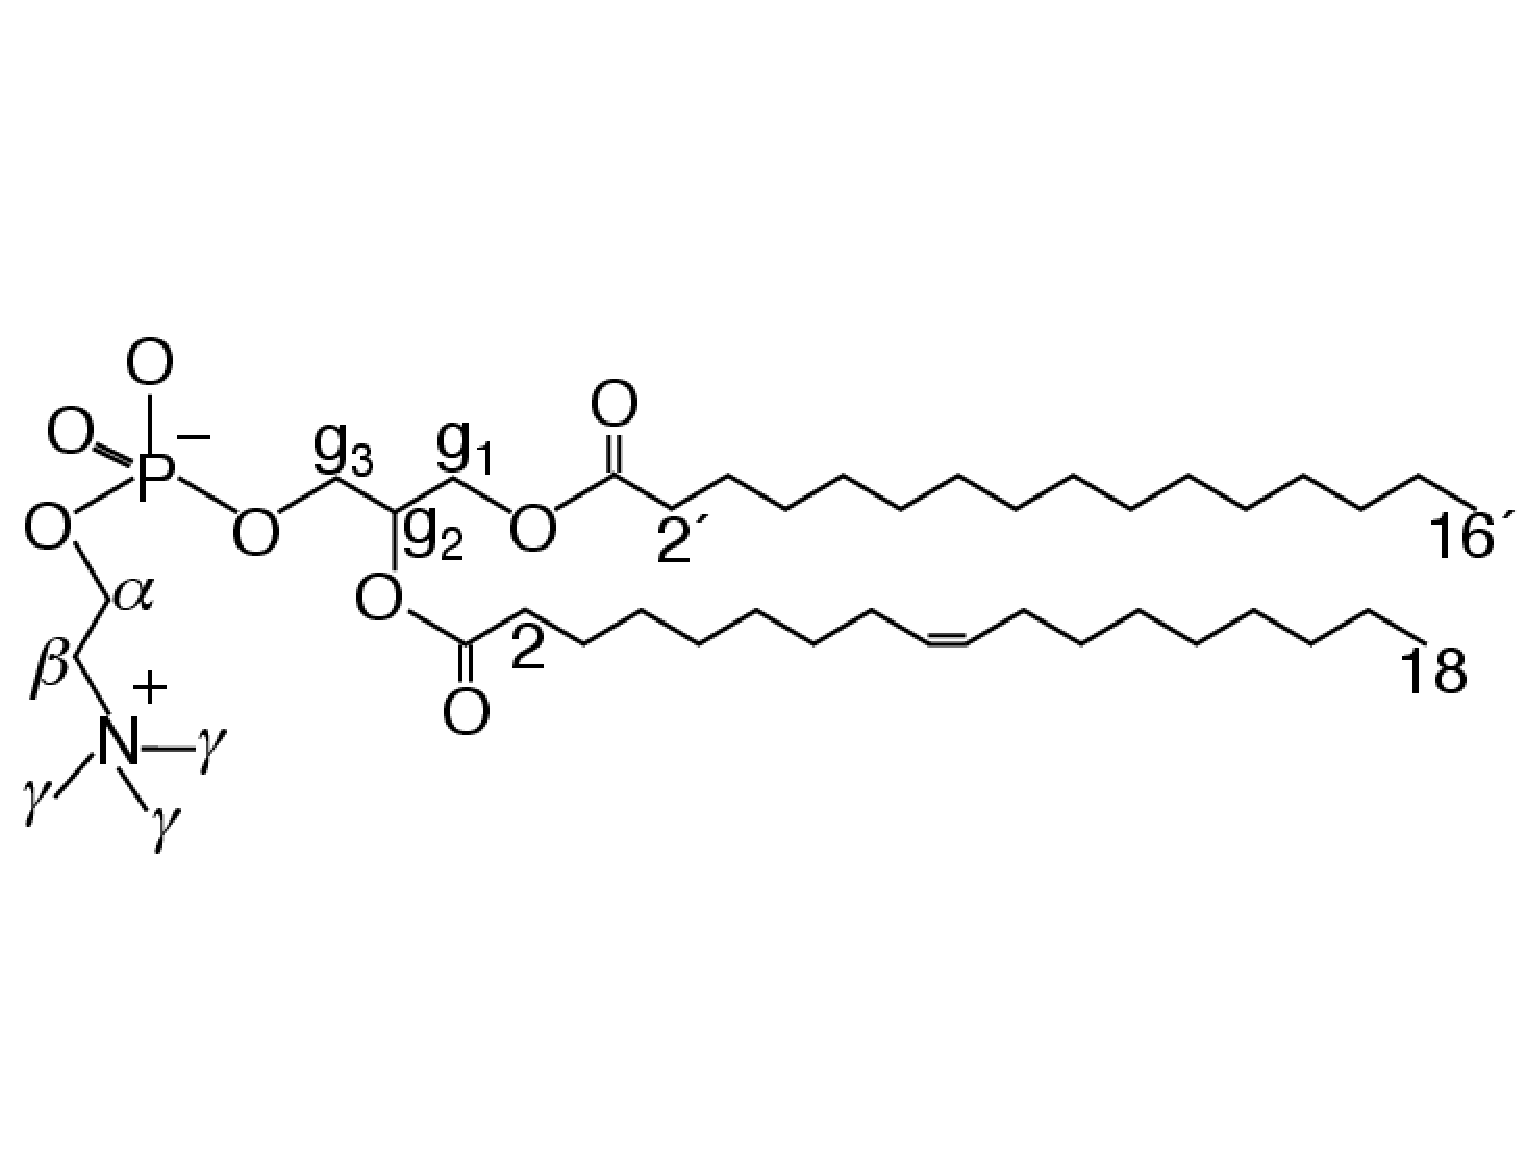
\includegraphics[width=8.6cm]{../Fig/POPCstructure.eps}

  \caption{\label{POPCstructure}
    Chemical structure of POPC.}
  
\end{figure}
The concept is based on the findings that the absolute value of the $\beta$ order parameter
increases and the $\alpha$ order parameter decreases with inceasing amount of penetrating 
charges~\cite{akutsu81,altenbach84,seelig87,scherer89}. 
From the simulation point of view the electrometer concept is particularly interesting since one
can directly compare the actual measurable quantity, i.e. order parameters, to the simulations.
In this work we compare the ion induced changes in phosphatidylcholine headgroup order parameters
between different simulation models to resolve the above discussed controversies in the literature.

%In this work we concentrate on the effect of Na$^+$ and Ca$^{2+}$ since those are widely discussed 
%ions in the simulation literature~\cite{pandit03,bockmann03,bockmann04,??}, and the experimental data is available~\cite{akutsu81,altenbach84}. 

In our recent work we showed that the experimental order parameters for choline and glycerol backbone were not
quantitatively reproduced by any available lipid model in fully hydrated conditions, however, the response of the choline order parameters
to the dehydration were qualitatively correct in all models and the response to the cholesterol  concentration
was correct for the CHARMM36 model~\cite{botan15}. In this work, we show that the qualitative response of order parameters
to penetrating cations is qualitatively correct but the partition of ions is too strong in all the studied models.


\section{Results and Discussion}
The effect of NaCl on the choline and glycerol bakcbone order parameters from experiments by Akutsu et al.~\cite{akutsu81}
and various simulations are shown in Fig.~\ref{ordPnacl}. 
The simulated systems are described in the table~\ref{IONsystems} and further details are given in Supplementary Information. 
The experimental results are shown for DPPC bilayer due to more extensive data set~\cite{akutsu81}, 
however the measurements for POPC gave essentially the same results~\cite{altenbach84}.

\begin{figure}[]
  \centering
  \includegraphics[width=8cm]{../Fig/OrderParameterIONSnaclSIGN.eps}
  \caption{\label{ordPnacl}
    Order parameters as a function of NaCl concentration from simulations 
     with the Berger, CHARMM36, MacRog and Orange force fields compared to the experiments
     by Akutsu et al.~\cite{akutsu81} and Altenbach et al.~\cite{altenbach84}. The signs are assumed to be the same as measured by Hong et al.~\cite{hong95a}, Hong et al.~\cite{hong95a} and Gross et al.~\cite{gross97}. 
     The experimental data for the effect of ions to the glycerol backbone is not found, thus only the values without ions are shown. 
     The straight line between the results with and without ions is plotted to guide the eye. 
   }
\end{figure}

\begin{figure}[]
  \centering
  \includegraphics[width=8cm]{../Fig/OrderParameterIONSCaCl.eps}
  \caption{\label{ordPcacl}
    Order parameters as a function of CaCl concentration from simulations 
     with the Berger 
%CHARMM36, MacRog 
and Orange force fields compared to the experiments by Akutsu et al.~\cite{akutsu81} and Altenbach et al.~\cite{altenbach84}. 
The signs are assumed to be the same as measured by Hong et al.~\cite{hong95a}, Hong et al.~\cite{hong95a} and Gross et al.~\cite{gross97}. 
     The effect of ions to the g1 and g2 were not measured, thus only the values without ions are shown. The straight line between the results with and without ions is 
     plotted to guide the eye. 
   }
\end{figure}

\begin{table*}[htb]
\centering
\caption{Simulated lipid bilayers with ions. The ion concentrations are the concentration of ions in buffer to solute the lipid bilayers and calculated as [ion]=(N$_{\rm ion} \times$[water])/N$_{\rm w}$, 
where [water]=55.5M. These correspond the concentrations reported in the experiments by Akutsu et al.~\cite{akutsu81}.}\label{IONsystems}
\begin{tabular}{c c c c c c c c c c c c}
%\hline
Force field & lipid & [Ion] mM & \footnote{The number of lipid molecules}N$_{\rm l}$   &  \footnote{The number of water molecules}N$_{\rm w}$   & \footnote{The number of Na$^+$ molecules}N$_{\rm Na}$  & \footnote{The number of Ca$^{2+}$ molecules}N$_{\rm Ca}$   &  \footnote{The number of Cl molecules}N$_{\rm Cl}$ & \footnote{Simulation temperature}T (K)  & \footnote{The total simulation time}t$_{{\rm sim}}$(ns) & \footnote{Time frames used in the analysis}t$_{{\rm anal}}$ (ns) & Files\\
\hline
Berger-POPC-07\cite{ollila07a}   &   POPC & 0          & 128 & 7290 & 0  & 0  & 0 & 298  & 270 & 240 & \cite{bergerFILESpopc}  \\
Berger-POPC-07\cite{ollila07a}, ionFF~\cite{??}\todoi{Appropriate reference for the ion model?}   &   POPC & 340 (NaCl) & 128 & 7202 & 44  & 0  & 44 &298  & 110 & 50 &?\todoi{Samuli put to Zenodo} \\
Berger-POPC-07\cite{ollila07a}, ionFF~\cite{??}\todoi{Appropriate reference for the ion model?}   &   POPC & 340 (CaCl$_2$) & 128 & 7157 & 0 & 44  & 88 &298 & 110 & 50 &?\todoi{Samuli put to Zenodo}  \\
\hline
CHARMM36\cite{klauda10}   & POPC & 0           & 72 & 2242 & 0  & 0 & 0 & 303  & 30 & 20 & \cite{charmm36filesSHORT} \\
CHARMM36\cite{klauda10}, ionFF~\cite{??}\todoi{Appropriate reference for the ion model?}   & POPC & 350 (NaCl)  & 72 & 2085 & 13  & 0 & 13 & 303  & 80 & 60 &?\todoi{Samuli put to Zenodo}\\
CHARMM36\cite{klauda10}, ionFF~\cite{??}\todoi{Appropriate reference for the ion model?}   & POPC & 690 (NaCl)  & 72 & 2085 & 26  & 0 & 26 & 303  & 80 & 60 &?\todoi{Samuli put to Zenodo} \\
CHARMM36\cite{klauda10}, ionFF~\cite{??}  & POPC & 950 (NaCl)  & 72 & 2168 & 37  & 0 & 37 & 303  & 80 & 60 &? \\
CHARMM36\cite{klauda10}, ionFF~\cite{??}\todoi{Appropriate reference for the ion model?}  & POPC & 1380 (NaCl)  & 72 & 2085 & 52  & 0 & 52 & 303  & 80 & 60 &?\todoi{Samuli put to Zenodo} \\
CHARMM36\cite{klauda10}, ionFF~\cite{??}\todoi{Appropriate reference for the ion model?}   & POPC & 2080  (NaCl)  & 72 & 2085 & 78  & 0 & 78 & 303  & 73 & 60 &?\todoi{Samuli put to Zenodo} \\
CHARMM36\cite{klauda10}, ionFF~\cite{??}   & POPC &  670 (CaCl$_2$)  & 72 & 2164 & 26  & 0 & 52 & 303  & 200  & 120 &? \\
\hline
MacRog\cite{maciejewski14}\todoi{DONE}  & POPC & 0 & 288 & 14400 & 0 & 0 & 0 & 310 & 90&40  &~\cite{macrogdehydFILES}  \\
MacRog\cite{maciejewski14}\todoi{DONE} , ionFF~\cite{??}\todoi{Appropriate reference for the ion model?}  & POPC & 100 (NaCl) & 288 & 14554 & 27 & 0 & 27 & 310 & 90&50  & \cite{macrogIONfiles} \\
MacRog\cite{maciejewski14}\todoi{DONE} , ionFF~\cite{??}\todoi{Appropriate reference for the ion model?}        & POPC &  210 (NaCl) & 288 & 14500 & 54 & 0 & 54 & 310 & 90&50  &\cite{macrogIONfiles}  \\
MacRog\cite{maciejewski14}\todoi{DONE} , ionFF~\cite{??}\todoi{Appropriate reference for the ion model?}        & POPC &   310 (NaCl) & 288 & 14446 & 81 & 0 & 81 & 310 & 90&50  & \cite{macrogIONfiles} \\
MacRog\cite{maciejewski14}\todoi{DONE} , ionFF~\cite{??}\todoi{Appropriate reference for the ion model?}        & POPC &   420 (NaCl) & 288 & 14392 & 108 & 0 & 108 & 310 & 90& 50  & \cite{macrogIONfiles}  \\
\hline
Orange, ionFF~\cite{??}\todoi{Samuli check the numbers}   &   POPC & 0 & 72 & 2880 & 0 & 0  & 0 & 298 & 60 & 50 &?\todoi{Jukka Määttä and Luca Monticelli, please let us know if we can share some files. This is unpublished model.}  \\
Orange, ionFF~\cite{??}\ &   POPC & 140 (NaCl) & 72 & 2866 & 7 & 0  & 7 & 298 & 120 & 100 &?  \\
Orange, ionFF~\cite{??}\todoi{Appropriate reference for the ion model?}   &   POPC & 510 (NaCl) & 72 & 2802 & 26 & 0  & 26 & 298 & 120 & 100 &?\todoi{Jukka Määttä and Luca Monticelli, please let us know if we can share some files through Zenodo. This is unpublished model.}  \\
Orange, ionFF~\cite{??}  &   POPC & 1000 (NaCl) & 72 & 2780 & 50 & 0  & 50 & 298 & 120 & 80 &? \\
%\hdashline
Orange, ionFF~\cite{??}\todoi{Appropriate reference for the ion model?}   &   POPC & 510 (CaCl$_2$)  & 72 & 2802 & 0 & 26  & 52 & 298 & 120 & 60 &? \todoi{Jukka Määttä and Luca Monticelli, please let us know if we can share some files. This is unpublished model.} \\
\hline
Slipid\cite{jambeck12}   &   DPPC & 0 & 128 &3840 & 0 & 0  & 0 & 323 & 150 & 100 &~\cite{slipidsFILES}  \\
Slipid\cite{jambeck12}, ionFF~\cite{??}\todoi{Andrea Catte, please let us know if you share some files through Zenodo}    &   DPPC & 150 (NaCl) & 600 & 18000 & 49 & 0  & 49 & 323 & 100 & 40 &?  \\
\end{tabular}
\end{table*} 

The most important observation is that the experimental order parameters for the headgroup and glycerol bakcbone g$_3$ segment 
are practically unhanged even though 1M NaCl concentration was added to the system. Thus, the presense of mM concentrations
of NaCl do not affect the structure of these parts of lipids. On the other hand, the presence of multivalent ions or 
charged amphiphiles changes the $\alpha$ and $\beta$ order parameters in a systematic way suggesting that the amount
and sign of charge penetrated into a bilayer can be measured from the changes of these parameters~\cite{akutsu81,altenbach84,seelig87,scherer89}.
This is known as the ''electrometer concept''. Thus, the most straightforward explanation for the experimental results shown
in Fig.~\ref{ordPnacl} is that the Na$^+$ and Cl$^-$ ions do not essentially penetrate into a phospholipid bilayer below 1M concentrations.

The response of order parameters to the NaCl concentration in simulations depends on the used model in Fig.~\ref{ordPnacl}:
The addition of NaCl leads to a significant changes for choline and $g_2$ and g$_3$ segments in glycerol bakcbone
in Berger and MacRog models, while only moderate changes are seen in CHARMM36 and Orange force fields.
The experimental data for glycerol backbone as a function of NaCl concentration is available only for the
g$_3$ segment. The changes in g$_1$ and g$_2$ are unlikely since all the other order parameters are unaffected
and $^1$H NMR data indicates that multivalent cations binding to phospholipid interact mainly with choline group
leaving glycerol backbone conformations intact~\cite{hauser76,hauser78}.


%Akutsu et al.~\cite{akutsu81} is shown in Fig.~\ref{ordPnacl} together with the results from 
%various simulations. The experiments were later on done also for POPC bilayer~\cite{altenbach84}, and the  
%results were essentially identical. The more extensive experimental data set DPPC bilayer is used here.

%The result is in line with the large number of experiments with different techniques where
%NaCl did not affect PC lipid bilayer properties with these concentrations~\cite{cevc90,binder02,petrache06,pabst07,filippov09}.

The core idea of the electrometer concept is that the decrease (increase) of $\beta$- and $\alpha$-carbon order parameters
is related to cation (anion) penetration into a lipid bilayer. 
It should be noted that in the original experiments the absolute value of $\beta$ order parameter was increasing with the presense of cations,
however it was shown later on that the $\beta$ order parameter is negative~\cite{hong95a,hong95b,gross97}, 
thus the value is actually increasing (becoming less negative).
The order parameter changes for  $\beta$- and $\alpha$-segments 
are plotted in Fig.~\ref{ordPions} in the presense of NaCl and CaCl$_2$ from experiments and different simulations. 
The clear decrease seen with CaCl$_2$ compared to the negligible effect of NaCl. Interpreted in terms of
electrometer concept, the result indicates that the Ca$^{2+}$ ions signifincantly penetrate into PC bilayer in contrast to 
Na$^+$~\cite{akutsu81,altenbach84}.

%The experimental results~\cite{akutsu81}, plotted in Fig.~\ref{ordPions} shows a distinct difference
%in behaviour as a function of ions: the choline order parameters were unaffected by the addition of NaCl, 
%whereas a systematic decrease was observed by the addition of CaCl$_2$. Following the electrometer
%concept this means that the binding constant for divalent Ca$^{2+}$ is higher than for monovalent Na$^+$
%which is in line with the large amount of experimental data with different techniques~\cite{cevc90,binder02,petrache06,pabst07,filippov09}.
\begin{figure}[]
  \centering
  \includegraphics[width=8cm]{../Fig/OrderParameterIONSchanges.eps}
  \caption{\label{ordPions}
    The change of order parameters for $\beta$ and $\alpha$ segments as a function of NaCl (left column) and CaCl$_2$ (right column) concentrations from simulations 
    and experiments by Akutsu et al.~\cite{akutsu81}. The signs of the order parameters without ions are taken from~\cite{hong95a,hong95b,gross97} and it is reasonable
    to assume that the sign do not change with concentrations repsented here~\cite{altenbach84}. Note that the $\beta$ order parameter with negative sign decreases here with cation
    penetration in contrast to measured absolute value increase in the origical studues~\cite{akutsu81,altenbach84}.
    Regarding the actual electrometer concept this not relevant, however. 
    The experimental accuracy of order parameter changes is much higher than the accuracy of quantitative values due to high resolution of $^2$H NMR spectroscopy~\cite{??}. 
   }
\todo{I have now added the new results with ORANGE (140mM and 1M) and CHARMM36 (950mM).
I think that based on the current results we cannot say that the CHARMM36 has too strong Na binding compared to experiments.
This conclusion was originally partly based on simulations with much higher concentration 
(see discussion at: http://nmrlipids.blogspot.com/2015/02/the-first-draft-of-ion-lipid.html?showComment=1423750867868\#c3435589938183508901).
The text should be modified accordignly. It would be reasonable also to run longer CHARMM36 simulations since the model seems to be quite close
to experiments. The new results did not change the conclusion about the Orange model.} \\
\todo{I have now also ran simulation with CaCl$_2$ using CHARMM36 and the results are in the figure.
The agreement with experiments is pretty good. The text should be modified accordingly.} \\
\todo{ I think that it would be very interesting to test the modified CHARMM ions: Venable et al. dx.doi.org/10.1021/jp401512z, J. Phys. Chem. B 2013, 117, 10183−10192.
According to the paper, these parameters improve the ion binding to the charged lipid bilayers. Even though I think that testing this would be highly relevant, I do not have
time to do it now.}
\end{figure}

The differences in NaCl behaviour between different models already seen in Fig.~\ref{ordPnacl} are seen more clearly in Fig.~\ref{ordPions} showing the changes.
\todo{The discussion about simulation results with CaCl$_2$ to be written once we have all the results.}



%It should be noted that when the electrometer concept was developed and original experiments done in 1980s, 
%the signs of the order parameters were unknown. When the signs were measured in 1990s it turned
%out that the $\beta$ order parameter was negative while the $\alpha$ order parameter was 
%positive~\cite{hong95a,hong95b,gross97}. This means that actually the both $\beta$ and $\alpha$
%order parameters are decreasing with penetrating charge (absolute values are increasing and decreasing, respectively), as seen in Figs.~\ref{ordPions}.


%is based on measuring the changes in the
%$\beta$- and $\alpha$-carbon order parameters as a function of ion concetration~\cite{akutsu81,seelig87,scherer89,semchyschyn04}.
%Thus the changes in these order parameters as function of NaCl and CaCl$_2$ concentrations in experiments and different simulations
%are plotted in Fig.~\ref{ordPions}. 

%The measured choline order parameters for DPPC as function of NaCl and CaCl$_2$~\cite{akutsu81} 
%are plotted in Fig.~\ref{ordPions}. 
%Also for the CaCl$_2$ experiments with POPC gives essentially similar results~\cite{altenbach84}.


%Also the results with Orange force field in Fig.~\ref{ordPions} shows a distinct difference between different salts:
%CaCl$_2$ significantly reduces the $\beta$- and $\alpha$-order parameters while significantly smaller or negligible effect is seen with NaCl. 
%Note, however, that in the Orange force field addition of Ca$^{2+}$ leads 
%to changes in order parameters that are larger than in experiments.

To study the correlation between order parameter changes and ion partitioning into a bilayer, 
suggested by the electrometer concept~\cite{akutsu81,altenbach84,seelig87,scherer89}, the density distributions as a function of membrane normal 
are shown in Fig.~\ref{IONdensCOMP} for lipids and cations from different simulation models. 
%to see if larger ion induced effects
%in choline order parameters correlates with ion binding also in simulation models.
\begin{figure}[]
  \centering
  \includegraphics[width=8cm]{../Fig/IONdensities.eps}
  \caption{\label{IONdensCOMP}
    Mass density profiles for lipids and ions from simulations with different force fields. 
    The lipid densities are divided with 100 to make them visible with the used y-axis scale.
  }
\todo{This figure is in progress, however, the main point can be seen. \\
- I think that we should use number densities instead of mass densities to make the difference between Na and Ca distributions more clear. 
Now the difference comparison is little bit distracted due to the different mass of the atoms. \\
- The lipid density from MacRog simulation is missing. Maybe Matti Javanainen could provide this?
If the data will be uploaded to Zenodo, it also trivial to calculate it with script. \\
- CONCENTRATION CALCULATION ISSUE FIXED, SEE http://nmrlipids.blogspot.com/2015/02/the-first-draft-of-ion-lipid.html?showComment=1423750867868\#c3435589938183508901. \\
The systems are here now with quite different concentrations so comparison is not straigthforward. One option would be to run simulations of all
systems with 150mM which would be close to physiological concentrations, and show the density distributions from those here. \\
- The CHARMM36 simulations with CaCl$_2$ is now done. With a first look it seems that the partition is similar or stronger than in Orange model
even though the order parameter change was much larger in the Orange model (see Fig.~\ref{ordPions}).
This would indicate that the different order parameter response in the Orange model would be due to the reaction of headgroup into
penetrating charge, not due to the difference in partition. However, this requires more detailed studies.
Since the CHARMM36 results are pretty good, it would be reasonable to run the simulations also with different concentrations.
The text should be updated accordingly. \\
- Figure editing will be finished (centering of the graphs, labels, etc.) will be done once the above issues have been sorted out.
 }
\end{figure}
It is evident from the figure that the Na$^+$ density peaks at the lipid bilayer interface are higher (indicating stronger ion binding) for the models
experiencing also larger changes in order parameters with NaCl concentration shown in Fig.~\ref{ordPnacl}. 
The both Na$^+$ binding affinity and order parameter changes are smallest, thus closest to the experiments, for the Orange model, and then incease 
in order CHARMM36, MacRog, and Berger having the highest binding affinity and order parameter changes.
%Simultaneously, it is evident from Figs.~\ref{ordPnacl} and~\ref{ordPions} that the order parameter decrease due to addition
%of NaCl is more pronounced in Berger and MacRog models compared to the CHARMM36 and Orange. 
Thus, the correlation between decreasing choline order parameters
and amount of penetrating cations (i.e. the electrometer concept) is also seen in simulations, independently of the quantitative quality of the used simulation model.

The most straightforward explanation for our results is that Na$^+$ ions do not practically penetrate into a PC lipid bilayer
with mM concentrations, thus the presense of NaCl does not affect the bilayer properties as observed in various experiments~\cite{akutsu81,altenbach84,clarke99,binder02,pabst07,filippov09}.
Consequently, the Na$^+$ penetration and concominant changes in order parameters, area per molecule and lateral diffusion 
seen in almost all simulation models would be artefact due to overestimated attraction between ions and lipid bilayer.
Even though this would also explain the absense of positive zeta potential in electrophoresis experiments~\cite{eisenberg79,tatulian87,manyes05,manyes06,klasczyk10},  
the presented data do not rule out the suggested possiblity of equal binding of Na$^+$ and Cl$^-$ ions~\cite{knecht13},
however, this equal binding should happen in such a way that the bilayer properties are unaffected.
Negligible binding of Na$^+$ with mM concentrations suggested here differs from the conclusions made from 
measurements of fluorescent probe dynamics~\cite{bockmann03,vacha09a,harb13}, membrane hardiness with AFM~\cite{manyes05,manyes06,fukuma07,ferber11,morata12} and calorimetry~\cite{bockmann03,klasczyk10}.
However, the fluorescent measurement results may arise from direct interactions between probe and ions, as already suggested by Filippov et al.~\cite{filippov09}. 
Further, the calorimetric results have been also interpreted to support negligible binding~\cite{cevc90}, and AFM result is relatively indirect, thus
there may be alternative explanations as well.

The effect of Ca$^{2+}$ on the $\alpha$ and $\beta$ order parameters is overestimated in all the simulation models, however,
qualitatively the change is correct, i.e. order parameters are decreasing.
The overestimation of the effect could be due to too strong partitioning or too sensitive headgroup model to the presense of ions.
\todo{The discussion should be finished when we have CHARMM results with CaCl$_2$.} \\
\todo{The $^1$H NMR experiments suggest that the N-$\beta$-$\alpha$-O dihedral is only in gaughe conformation in the absense of ions, but
in the presense of multivalent ions there would be also anti conformations present [Hauser et al. BBA {\bf 508}, 450 (1978), Hauser et al. Chem. Phys. Lipids {\bf 29}, 103 (1981)].
I think that we should check if this happens in simulations.}

%In conclusion, our results show that the Na$^+$ association to PC bilayer is significantly too strong in the Berger and MacRog models,
%while Orange and CHARMM36 force fields predict more realistic binding affinity. Since some modest changes are also seen in 
%Orange and CHARMM36 results, more careful simulation studies would be needed to judge if the Na$^+$ association is slightly 
%too strong also in these  models. The stonger Na$^+$ ion association in GROMOS based force fields compared to CHARMM based force 
%has been already reported in the literature~\cite{berkowitz06,cordomi09,valley11,berkowitz12,sachs04,valley11},
%however the novelty of this work in this respect is that we make a direct comparison
%to the experiments which can be used as measure for the model quality. 

The origin for suggested inaccuracies in lipid-ion interactions in simulation models us unknown. 
In principle, the incorrect choline structure~\cite{botan15}, lack of polarizability~\cite{leontyev11} or
the used water model could cause such results. The effect of changes in lipid and ion model ot the ion
partition is discussed in supplementary material.
\todo{In the Orange simulation only lipid model is changed, respect to Berger, and Jukka tested the effect
of 0.7 charge scaling for Na ion (suggested by Leontyev et al.~\cite{leontyev11} to compensate to the lack 
of electronic polarizability in the model). I think we should discuss these things in supplementary material.
Even though we cannot be fully conclusive, there is some essential information also in these results.} 

%From the technical point of view it is interesting to note that the same ion model is used in the Berger and Orange simulation, only difference 
%being in the lipid model, indicating that the partitioning can be strongly reduced just by modifying the lipid
%model parameters. 

%In situations where a positive charge penetrates into a bilayer (e.g. cationic surfactant~\cite{scherer89} or multivalent ion~\cite{akutsu81}) 
%a decrease in choline order parameters is observed in experiments, as also seen in CaCl$_2$ results in Fig.~\ref{ordPions}.
%Also in all simulations analyzed in this work where cation is penetrating into a bilayer, the choline order parameters
%decrease as seen in Fig.~\ref{ordPions}. However, in the case of CaCl$_2$ the decrease in too pronounced in 
%simulations which may arise from too strong partitioning of Ca$^{2+}$ or overestimated influence of charge on lipid conformation.

\section{Conclusions}
We have compared phosholipid bilayer interactions with NaCl and CaCl$_2$ between different molecular dynamics simulation
models and $^2$H NMR experiments. The comparison led to the following conclusions

- The most straighforward explanation for the various experimental obsevations is that there is no Na$^+$ ion binding
into the phospholipid bilayer with mM concentrations, in constrast to Ca$^{2+}$ which specifically binds.

- The Na$^+$ is overestimated in almost all molecular dynamics simulation models, however, from the publicly available
models the CHARMM36 has the most realistic description.

- The electrometer concept suggesting connection between $\alpha$ and $\beta$ order parameter decrease and
cation partitioning~\cite{akutsu81,altenbach84,seelig87,scherer89} works also in simulations, despite of inaccuracies in actual atomistic resolution structures. 

%Our discussion gives further support to the idea that choline orientation and ion partitioning can
%be experimentally measured by using the choline group order parameters as suggested in the series of
%publications by Seelig and co workers.
%However, we have updated the details of the relation by including the information about 
%the sings.

- \todo{Final conclusions about the structural response to be written once we have all the results} 


%In conclusion, the penetrating induced decrease in order parameters can be seen in all models
%independently of the detailed molecular structure in the model, corresponding to the dehydration case
%where increase was seen in all models. The most likely explanation is that, despite of the structural model, the choline group
%orients more parallel to the membrane normal with penetrating cations. In contrast to the dehydration results,
%we are not aware of experimental data for the glycerol order parameters as a function of penetrating ions. 
%Furher, our results show that the Na$^+$ partitioning into a PC bilayer with Berger model is a
%simulation artefact, thus the research lines based these results should be taken with caution.


%This work has been done, and will be progressed, as an open collaboration through nmrlipids.blogspot.fi.






%Similar significant structural changes in the headgroup region are seen upon the addition
%of sodium and calcium ions in the Berger model. This contradicts with the experiments where
%sodium does not change the headgroup structure and the changes observed for calcium are different from those seen in simulations.
%These results indicate that the changes in the headgroup structure due to a permeating charge are not correct
%in the Berger model and, in particular, that sodium ions penetrating the headgroup region is erroneous.

This work has been, and will be further, progressed and discussed through the blog: nmrlipids.blogspot.fi. 
Everyone is invited to join the discussion and make contributions through the blog. 
The manuscript will be eventually submitted to an appropriate scientific journal. 
Everyone who has contributed to the work through the blog will be offered 
coauthorship. For more details see: nmrlipids.blogspot.fi.   

{\bf Acknowledgements: }
OHSO acknowledges Tiago Ferreira for very useful discussions, the Emil Aaltonen foundation for financial support, Aalto Science-IT project and CSC-IT Center for Science for computational resources. 


\newpage

\appendix
\begin{center}
{\bf SUPPLEMENTARY INFORMATION}
\end{center}

\section{methods}

\subsection{Simulated systems}
All simulations are ran with a standard setup for planar lipid bilayer in zero tension
with periodic boundary conditions with Gromacs software package (version numbers 4.5-X-4.6.X).
%The number of molecules, temperatures and the length of simulations for all the fully 
%hydrated lipid bilayer simulations are listed in Table~\ref{systems}. Full simulation
%details for all simulations are given the next section.

%For intitial configuration of the simulations with NaCl and CaCl$_2$, the required number of randomly placed water molecules were replaced by 
%ions in fully hydrated simulations. 
%The molar concentration was calculated as ??. 
%The number of different molecules, temperatures and 
%the length of simulations for all the ion containing simulations are show in Table~\ref{IONsystems}.


%the POPC bilayer was solvated with 7202 water molecules, 44 Na$^+$ and Cl$^-$ ions,
%corresponding roughly to [NaCl] $\approx$ 200~mM. For simulations with CaCl$_2$, the POPC bilayer was solvated with 
%7157 water molecules, 44 Ca$^{2+}$ and 88 Cl$^-$ ions, corresponding roughly to [CaCl$_2$] $\approx$ 200~mM. 
%The order parameters were calculated from the last 50~ns of a trajectory
%totalling 110~ns. 


\subsection{Simulation details}
\subsubsection{Berger}
The simulation without ions is the same as in~\cite{botan15}. The starting structures for simulations with ions is
made by replacing water molecules with appropriate amount of ions under study.
\todo{Samuli, finalize and check the methods.}

The Berger force field was used for the POPC~\cite{berger97}, with the dihedral potential next to the double bond 
taken from~\cite{bachar04}. The simulations are identical to previous publications~\cite{ollila07a,ferreira13,ferreira15}.
Timestep of 2~fs was used with leap-frog integrator. Covalent bond lengths were constrained with LINCS algorithm~\cite{hess97,hess07}. 
Coordinated were written every 10~ps. PME with real space cut-off 1.0~nm was used 
for electrostatics. Plain cut-off was used for the Lennart-Jones interactions with a 1.0~nm cut-off.
The neighbour list was updated every 5th step with cut-off 1.0~nm. Temperature was coupled separately
for lipids and water to 298~K with the velocity-rescale method~\cite{bussi07} with coupling constant 0.1~ps$^{-1}$.
Pressure was semi-isotropically coupled to the athmospheric pressure with the Berendsen method~\cite{berendsen84}.


\subsubsection{CHARMM36}
The simulation without ions is the same as in~\cite{botan15}. The starting structures for simulations with ions is
made by replacing water molecules with appropriate amount of ions under study.
\todo{Samuli, finalize and check the methods.}

Timestep of 1~fs was used with leap-frog integrator. Covalent bonds with hydrogens were constrained with LINCS algorithm~\cite{hess97,hess07}. 
Coordinated were written every 5~ps. PME with real space cut-off 1.4~nm was used 
for electrostatics. Lennart-Jones interactions were switched to zero between 0.8~nm and 1.2~nm.
The neighbour list was updated every 5th step with cut-off 1.4~nm. Temperature was coupled separately
for lipids and water to 303~K with the velocity-rescale method~\cite{bussi07} with coupling constant 0.2~ps.
Pressure was semi-isotropically coupled to the athmospheric pressure with the Berendsen method~\cite{berendsen84}.

\subsubsection{MacRog}
\todo{DONE}
The simulation parameters are identical to those employed in our earlier study~\cite{botan15} for the full 
hydration and dehydration simulations. The initial structures with varying amounts of NaCl were constructed from an 
extensively hydrated bilayer by replacing water molecules with ions using the gromacs tool genion. Even at the highest 
considered salt concentration, the amount of water molecules per lipid after this replacement process was still greater than 50.

\subsubsection{Orange}
\todo{Jukka Maatta and Luca Monticelli, please deliver as much details as you can.}

\subsubsection{Slipids}
The simulation without ions is the same as in~\cite{botan15}.
\todo{DONE}

For the simulations with ions, the starting DPPC lipid bilayer, which was built with the online CHARMM-GUI
(http://www.charmm-gui.org/), contained 600 lipids, 30 water molecules/lipid, Na+ and Cl- ions (150 mM NaCl). 
The TIP3p water model was used to solvate the system. AA MD simulations of DPPC lipid bilayers were performed 
at ten different temperatures (283, 298, 303, 308, 312, 313, 314, 318, 323, and 333 K) using the GROMACS software 
package version 4.5.5 and the Stockholm lipids (Slipids) force field parameters for phospholipids. After energy 
minimization and a short equilibration run of 50 ps (time step 1fs), 100 ns production runs were performed using 
a time step of 2 fs with leap-frog integrator. All covalent bonds were constrained with the LINCS
algorithm. Coordinates were written every 100 ps. PME with real space cut-off at 1.0 nm was used for Coulomb 
interactions. Lennard-Jones (LJ) interactions were switched to zero between 1.0 nm and 1.4 nm. The neighbour 
lists were updated every 10th step with a cut-off of 1.6 nm. Temperature was coupled separately for upper and 
bottom leaflets of the lipid bilayer, and for water to one of the temperatures reported above with the Nosè-Hoover 
thermostat using a time constant of 0.5 ps. Pressure was semi-isotropically coupled to the atmospheric pressure 
with the Parrinello-Rahman barostat using a time constant of 10 ps.
The last 40 ns of each simulation was employed for the analysis of DPPC choline and glycerol backbone order parameters.

\subsection{analysis}
The order parameters were calculated from simulation trajectories directly applying the equation
$S_{{\rm CH}}=\frac{3}{2} \langle \cos^2 \theta-1 \rangle$. For united atom models the hydrogen locations
were regenerated for each molecule in each frame after the simulation trajectory was created.
??The statistical error estimate for each order parameter calculated from simulation was roughly
0.01, which is much smaller than the differences discussed in this work.??


%Testing of the effect of changing the ion model and accounting of electronic polarization in lipid-ion interactions
%-Jukka
\subsection{Effect of ion model and polarization}

 We also tested if different ion models and implicit accounting of polarization would affect ion binding.
 Changing the model description from Berger-DPPC-98~\cite{Marrink98} and Gromos ion
 parameters~\cite{??}\todoi{Appropriate reference for the ion model?} to OPLS-AA compatible
 Berger-DPPC-06~\cite{tieleman06} and \r{A}qvist ions~\cite{Aaqvist90} results in slightly decreased ion binding affinity
 as seen from the density plots in Figure \ref{ionnotscaled}~\cite{DPPCBergerNaCl, DPPCBergerOPLS06NaCl}. The failure
 of Gromos ions to properly account ion-ion and ion-water binding propensities of sodium and chloride ions has been
 reported previously~\cite{Reif13}. The \r{A}qvist ions have been parameterized in aqueous solutions with good agreement
 to experimental energies~\cite{Aaqvist90}. Yet, the binding affinity of ions to lipid bilayers has not been
 calibrated - instead it is assumed to work based purely on forces obtained using combination rules. Compared to Gromos
 ions \r{A}qvist parameters are better, yet sodium overbinding still occurs.

To take account for polarization effects in non-polarizable models, Leontyev et al.~\cite{leontyev11} have suggested
that ion charges should be scaled by a factor of 0.7. We scaled the charges of both Gromos and \r{A}qvist ions. 
After scaling the order parameter changes due to ions and ion affinity into a bilayer of both ion models is decreased, see
Figs. \ref{OPchangesSCALED}, \ref{ionnotscaled} and \ref{ionscaled}~\cite{DPPCBergerNaClscaled, DPPCBergerOPLS06NaClscaled}. The intuitive explanation is that by
scaling the partial charges the charge discrepancy between the ion and water partial charges is decreased. This means
that there is a lesser driving force for ions to bind to the highly-charged phosphate group. Furthermore, with
Berger-DPPC-06 and scaled Åqvist ions (Q=0.7) we obtain that there is only very weak binding of sodium to DPPC as
observed experimentally (right side of Figure \ref{ionscaled}). In scaled models the order parameter changes 
are also small. However, the ion concentraion is also small. To be fully conclusive, if the affinity can be fixed by scaling
we need to run simulations also with large concentrations.


The results indicate that the polarization effect actually improves ion binding affinities irrespectively of the model.
However, the drawback of the scaled charges is that the total charge of the simulation box is non-zero whenever
counterions and charged molecules are present. This may cause simulation artefacts. Even though in methods such as
PME the residual charge does not affect the forces (and thus nor dynamics), it still has an effect to the energies.
This is because the potential from the residual charge is 'smeared in the box' and so depends on the possibly
fluctuating (at least in NPT conditions) volume of the simulation box. 

\begin{figure*}[]
  \centering
  \includegraphics[width=\textwidth]{../Fig/OrderParameterIONSchangesSCALED.eps} %https://zenodo.org/record/16319/files/density.png
  \caption{\label{OPchangesSCALED}
    Order parameter changes in scaled and non-scaled models. The Berger-OPLS compatible model results are missing since there are
    no results without ions for this.
}
\end{figure*}


\begin{figure*}[]
  \centering
  \includegraphics[width=0.49\textwidth]{../Fig/ionnotscaledberger98.eps} %https://zenodo.org/record/16319/files/density.png
  \includegraphics[width=0.49\textwidth]{../Fig/ionnotscaledberger06.eps} %https://zenodo.org/record/16484/files/density.png
  \caption{\label{ionnotscaled}
    Density plots of DPPC bilayer and ions. DPPC density has been scaled down by a factor of 100 for clarity. Left: Berger-DPPC-98 model with Gromos ions. Right: Berger-DPPC-06 model with \r{A}qvist ions.
}
\end{figure*}
%Raw data in .xvg format for this figure can be found at
%https://zenodo.org/record/16319/files/ and https://zenodo.org/record/16384/files/

\begin{figure*}[]
  \centering
  \includegraphics[width=0.49\textwidth]{../Fig/ionscaledberger98.eps} %https://zenodo.org/record/16320/files/density.png
  \includegraphics[width=0.49\textwidth]{../Fig/ionscaledberger06.eps} %https://zenodo.org/record/16485/files/density.png
  \caption{\label{ionscaled}
   Density plots of DPPC bilayer and polarization corrected ions, where ion charges are scaled by 0.7. DPPC density has been scaled down by a factor of 100 for clarity. Left: Berger-DPPC-98 model with scaled Gromos ions. Right: Berger-DPPC-06 model with scaled \r{A}qvist ions.
   }
\end{figure*}
%Raw data in .xvg format for this figure can be found at
%https://zenodo.org/record/16320/files/ and https://zenodo.org/record/16385/files/



%The order parameters calculated from previously published quadrupolar splitting data were calculated using 
%the equation $|S_{{\rm CD}}|=0.00784 \times \Delta \nu_Q$, where $\Delta \nu_Q$ is the quadrupolar splitting measured
%by $^2$H NMR (for more details see~\cite{seelig77c} and supplementary information).
%The order parameters measured with $^{13}$C NMR were calculated from dipolar splitting by using equation
%$|S_{{\rm CH}}|=\frac{4\pi\langle r_\mathrm{CH}^3 \rangle}{\hbar \mu_0 \gamma_h \gamma_c} d_\mathrm{CH}$, where
%$d_\mathrm{CH}$ is the measured dipolar splitting and
%values between 20.2-22.7 kHz were used for $\frac{4\pi\langle r_\mathrm{CH}^3 \rangle}{\hbar \mu_0 \gamma_h \gamma_c}$,
%depending on the original authors~\cite{hong95a,gross97,dvinskikh05,ferreira13} (for more discussion see supplementary material).




%The results for choline order parameters as a function of CaCl$_2$ from simulations and experiments
%in Fig.~\ref{ordPions} shows a significant decrease in both cases, however the decrease is more pronounced
%in simulations, indicating too high Ca$^{2+}$ partitioning of too strong effect to the order parameters
%in simulations. Also the decrease in order parameters in simulations with penetrating Na$^+$ ions (MacRog and Berger)
%is in qualitative agreement with experiments where penetrating positive ions are studied, Ca$^{2+}$ by Akutsu et al~\cite{akutsu81} also
%shown in Fig.~\ref{ordPions} and anionic surfactants by Scherer et al.~\cite{scherer89}.

%By comparing Figs~\ref{ordPnacl},~\ref{ordPions} and ~\ref{IONdensCOMP} it becomes clear that Na$^+$ binding is stronger (Fig. 4) in the force fields in which the 
%Na$^+$-induced changes in the order parameters are larger (Figs.~\ref{ordPnacl} and~\ref{ordPions}), i.e., in Berger and MacRog. In CHARMM36 and Orange, in which 
%the Na$^+$-induced changes in order parameters are smaller, also the partitioning of Na$^+$ is significantly less. It seems that the correlation between ion binding and order parameter 
%changes that was suggested from the NMR experiments~\cite{akutsu81,seelig87} can be reproduced in MD simulations. 

%In simulations the ion induced changes in the order parameters shown in Figs.~\ref{ordPnacl} and ~\ref{ordPions} depends
%on the used model: NaCl induces a dramatic decrease of the $\beta$- and $\alpha$-carbon order parameters in Berger and MacRog models
%while in CHARMM36 and Orange force fields only small or nonexistent changes are induced.
%The order parameter results are in with the ion distribution results in Fig.~\ref{IONdensCOMP}
%showing that signifanct fraction of Na$^+$ ions is located in the bilayer region
%for the MacRog and Berger models, while the ion penetration is much less for the
%Orange and CHARMM36. 

%The order parameters calculated from simulations with the Berger and MacRog force fields 
%for $\beta$ and $\alpha$ were clearly decreased by the presence of NaCl. Also order parameters
%for g$_3$ and g$_2$ were affected. The decrease of  $\beta$ and $\alpha$ order parameters
%is the signature of penetrating positive charges in the experiments, and indeed, the ion density
%distrubutions show that for both force fields a significant amount of Na$^+$ is located
%in the bilayer region. Slight decrease in  $\beta$ and $\alpha$ order parameters with 
%NaCl is also observed in CHARMM, and even less in the Orange. This observation is also
%in line with the density distributions of ions which show that CHARMM has some bound ions, Orange has less,
%and both have much less compared to the Berger and MacRog models. 

%The simulation results
%are in line with previous works~\cite{??}. As a conclusion, the results strongly indicate that the
%partitioning of Na$^+$ is strongly overestimated in the Berger and MacRog models, and also significantly
%overestimated in the CHARMM model. There seems to be weak partitioning present also in the Orange model,
%however to conclude if this is too strong or not more data should be generated. This is not done since the 





\onecolumngrid
\listoftodos

\bibliographystyle{apsrev}
\bibliography{refs}


\end{document}
